\section{Ajuste e interpretação de dados de temperatura}\label{sec:temperatura}

\subsection{Por que esta grandeza?}

A temperatura do ar é uma das grandezas termodinâmicas mais familiares no cotidiano e na experimentação científica elementar.

Frequentemente, em cursos introdutórios de física e engenharia, assume-se como premissa tácita que grandezas contínuas se comportam de forma gaussiana. Contudo, a grandeza física ``temperatura'' não determina, por si só, uma distribuição normal. A série agregada ao longo de vários anos incorpora fortes efeitos sazonais e transições de massas de ar que geram a sobreposição de populações com médias e variâncias distintas.

Este segundo exemplo desempenha um papel pedagógico complementar ao estudo da velocidade do vento. Enquanto no vento investigou-se a restrição de suporte e a assimetria positiva, na temperatura examina-se até que ponto uma distribuição aproximadamente simétrica justifica o abandono da distribuição normal em favor de uma família flexível de quatro parâmetros, ensinando o estudante a formular e testar criticamente essa hipótese.

\subsection{Definição do recorte temporal}

A análise da série plurianual completa revela uma variação sazonal evidente, que inviabiliza um modelo único para todo o ano sem estratificação. Para manter um recorte físico e temporal mais homogêneo, selecionou-se a temperatura média diária do mês de julho. O recorte contempla $768$ observações diárias válidas, distribuídas ao longo de 25 invernos (2000 a 2024).

A escolha de julho foi estabelecida \textit{a priori}, com base em um critério climatológico (o auge do inverno no Centro-Oeste brasileiro), e não por meio de uma varredura exploratória em busca do mês com maior aderência à normal ou à GLD. A restrição ao calendário atenua a heterogeneidade entre estações do ano, embora não elimine a dependência entre dias adjacentes nem a variabilidade interanual. O modelo ajustado deve ser interpretado como a caracterização probabilística das temperaturas médias diárias observadas em julho naquela estação meteorológica.

A figura~\ref{fig:temp_sazonalidade} ilustra o ciclo anual da temperatura na estação por meio da distribuição mensal e destaca a série do mês de julho. O painel (b) mostra também que alguns invernos, como os de 2004 e 2017, tiveram dias bem mais frios que os demais.

\begin{figure}[htbp]
\centering
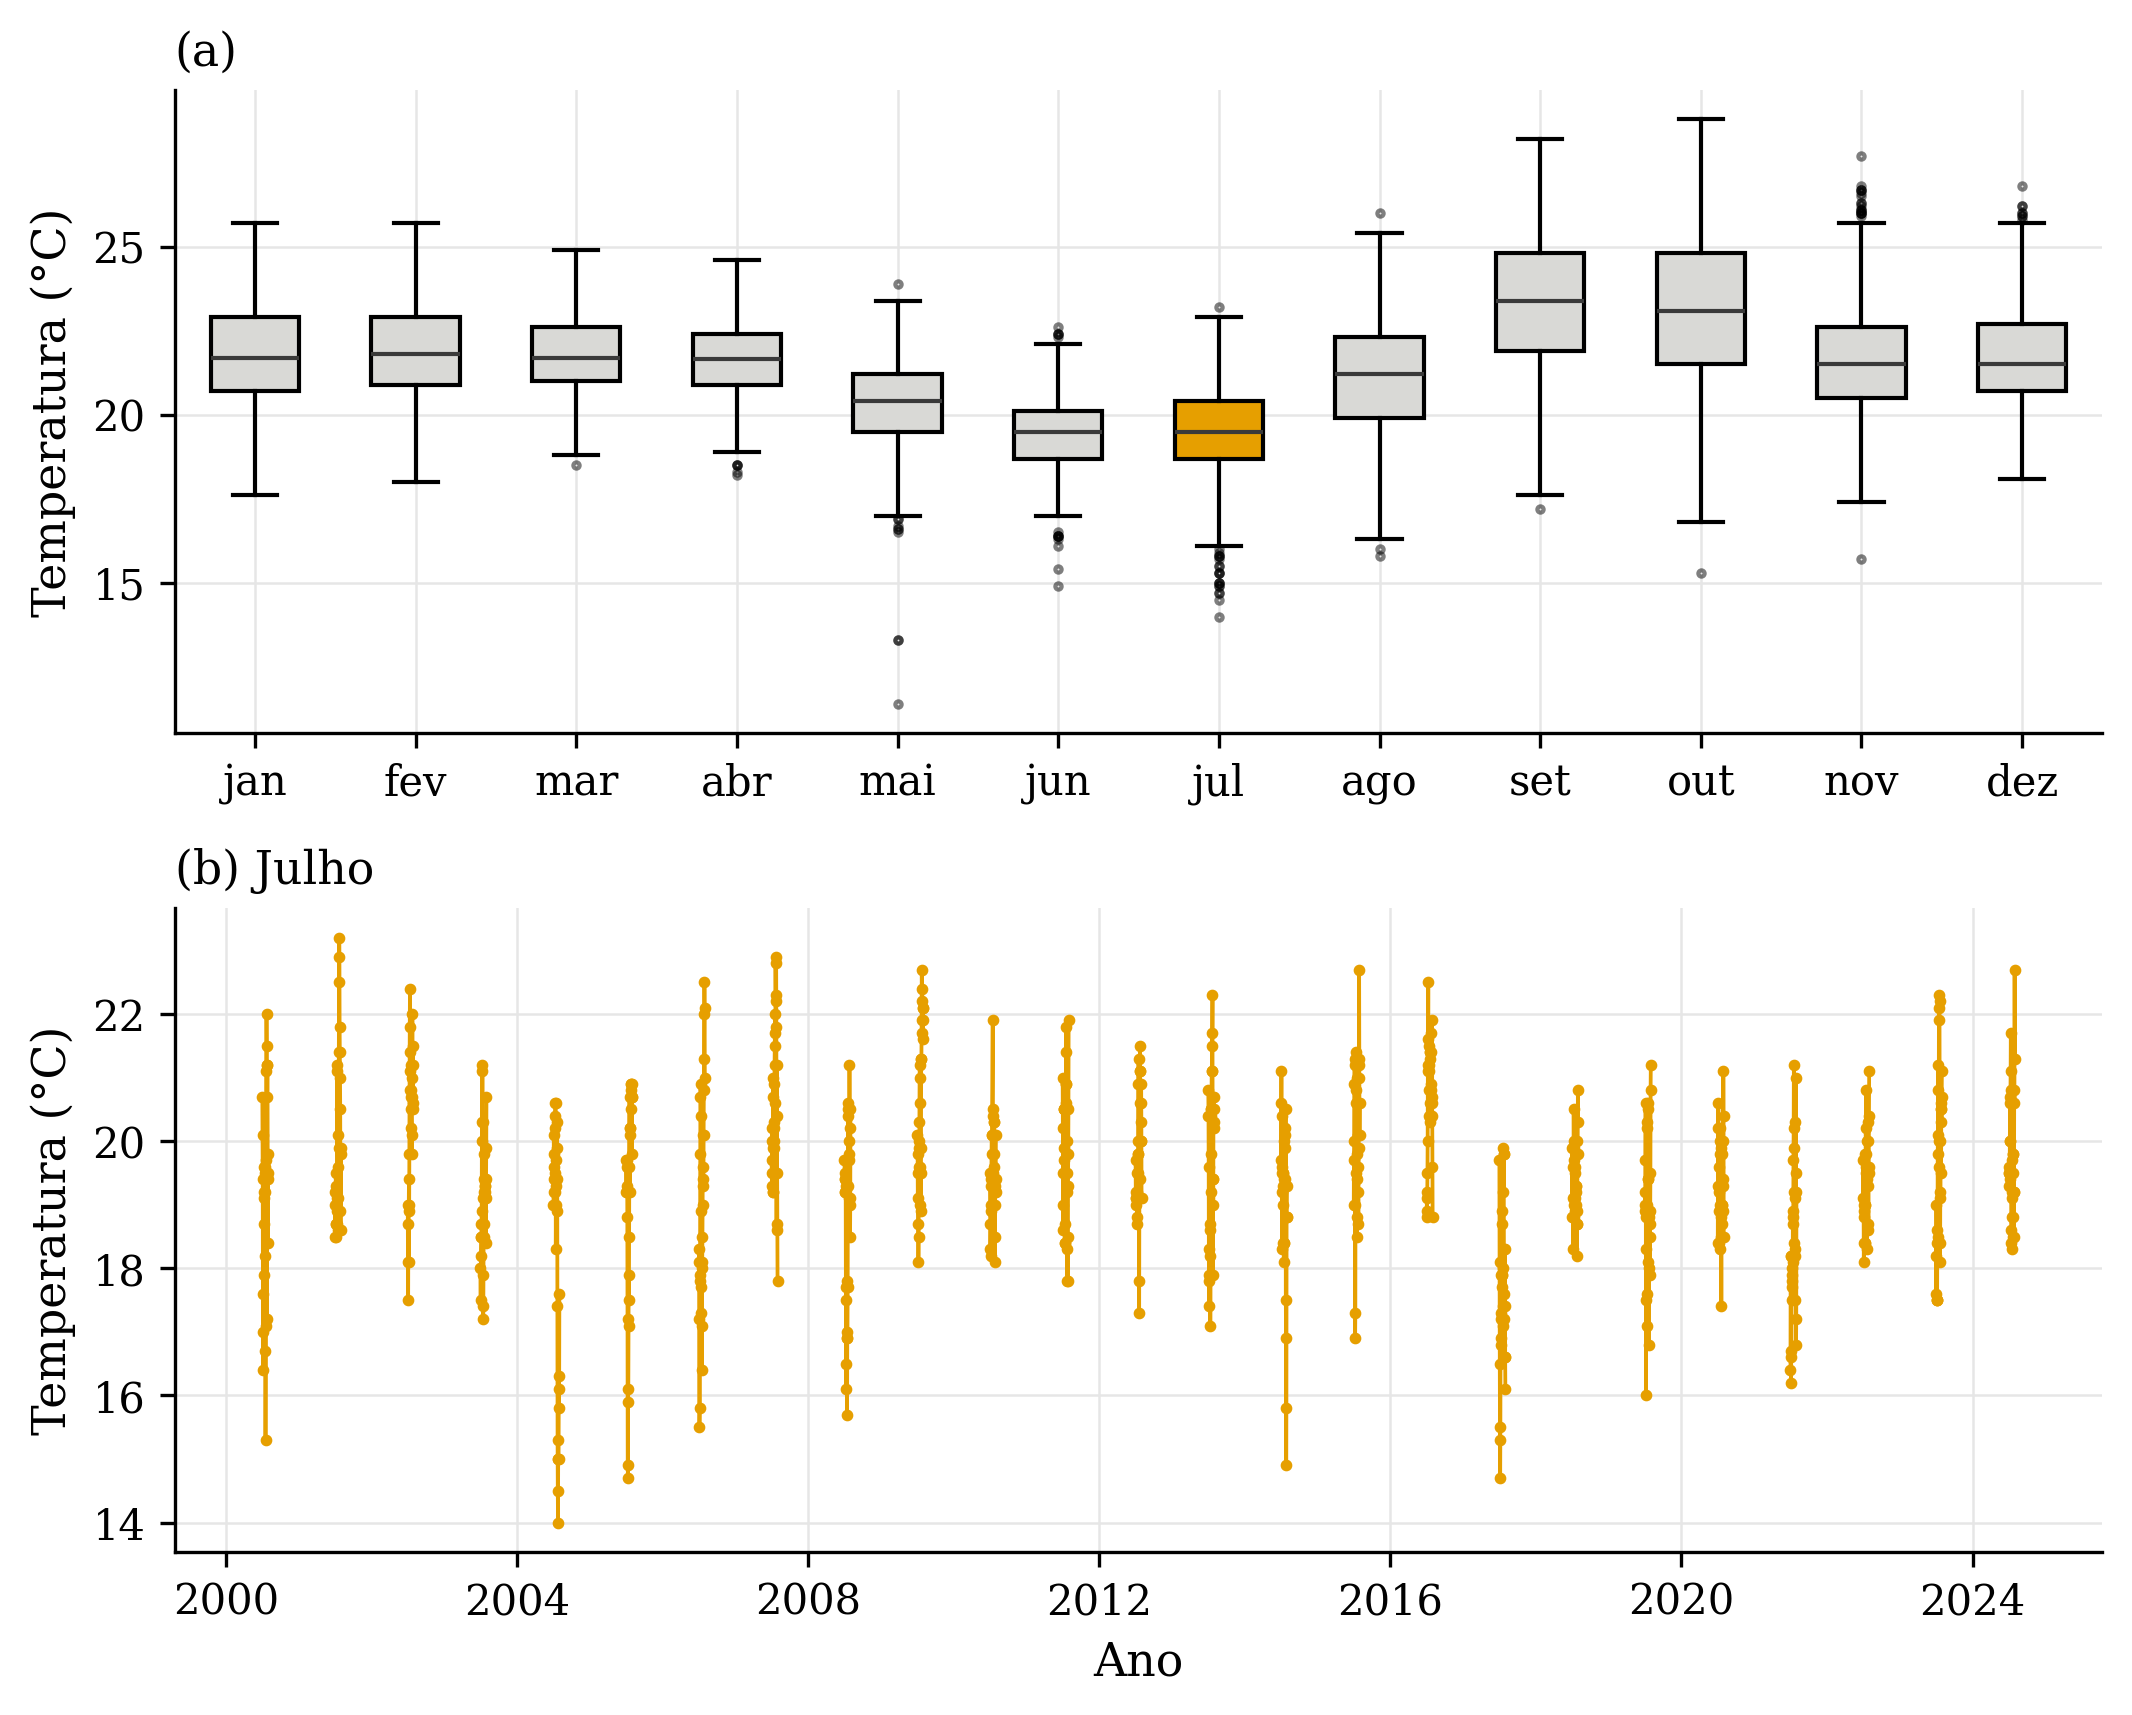
\includegraphics[width=0.85\textwidth]{figura4_temperatura_sazonalidade_pt.png}
\caption{Temperatura média diária na estação A001, com (a) a distribuição por mês, destacando julho, e (b) a série das temperaturas de julho, de 2000 a 2024.}
\label{fig:temp_sazonalidade}
\end{figure}

\subsection{Ajustes, gráficos e métricas}

A amostra de julho (tabela~\ref{tab:descritiva}) apresenta temperatura média de $19,409\,^\circ\text{C}$, desvio padrão de $1,466\,^\circ\text{C}$ (com divisor $n$), assimetria moderadamente negativa ($-0,482$) e curtose de Pearson de $3,717$, isto é, um excesso de $0,717$ em relação à normal. Os quantis empíricos de 5\%, 50\% e 95\% são $16,84\,^\circ\text{C}$, $19,50\,^\circ\text{C}$ e $21,70\,^\circ\text{C}$, respectivamente.

Aplicando o mesmo protocolo da seção~\ref{sec:vento}, comparou-se o modelo normal, com parâmetros de máxima verossimilhança $\widehat{\mu} = 19,409\,^\circ\text{C}$ e $\widehat{\sigma} = 1,466\,^\circ\text{C}$, com a GLD-FKML ajustada pelo método dos momentos com a biblioteca \texttt{pyglam}, que resultou em $\widehat{\boldsymbol\lambda} = (19,538;\, 1,071;\, 0,018;\, 0,184)$.

As discrepâncias quantílicas são reportadas diretamente na unidade física ($\Delta_p$, em $^\circ$C). A tabela~\ref{tab:desempenho_temperatura} apresenta os diagnósticos comparativos e a figura~\ref{fig:diagnosticos_temperatura} sintetiza a sobreposição das densidades, as funções acumuladas e o gráfico Q-Q.

\begin{table}[htbp]
\centering
\caption{Desempenho dos modelos ajustados às temperaturas médias diárias de julho. As diferenças de quantis $\Delta_p$ estão em $^\circ$C.}
\label{tab:desempenho_temperatura}
\begin{tabular}{lccccc}
\toprule
\textbf{Modelo} & \textbf{Parâmetros} & \textbf{$D_n$} & \textbf{$\Delta_{0,05}$} & \textbf{$\Delta_{0,50}$} & \textbf{$\Delta_{0,95}$} \\
\midrule
Normal & 2 & 0{,}064 & +0{,}163 & -0{,}091 & +0{,}120 \\
GLD-FKML & 4 & 0{,}041 & +0{,}025 & +0{,}002 & -0{,}058
\unskip \\
\bottomrule
\end{tabular}
\end{table}

\begin{figure}[htbp]
\centering
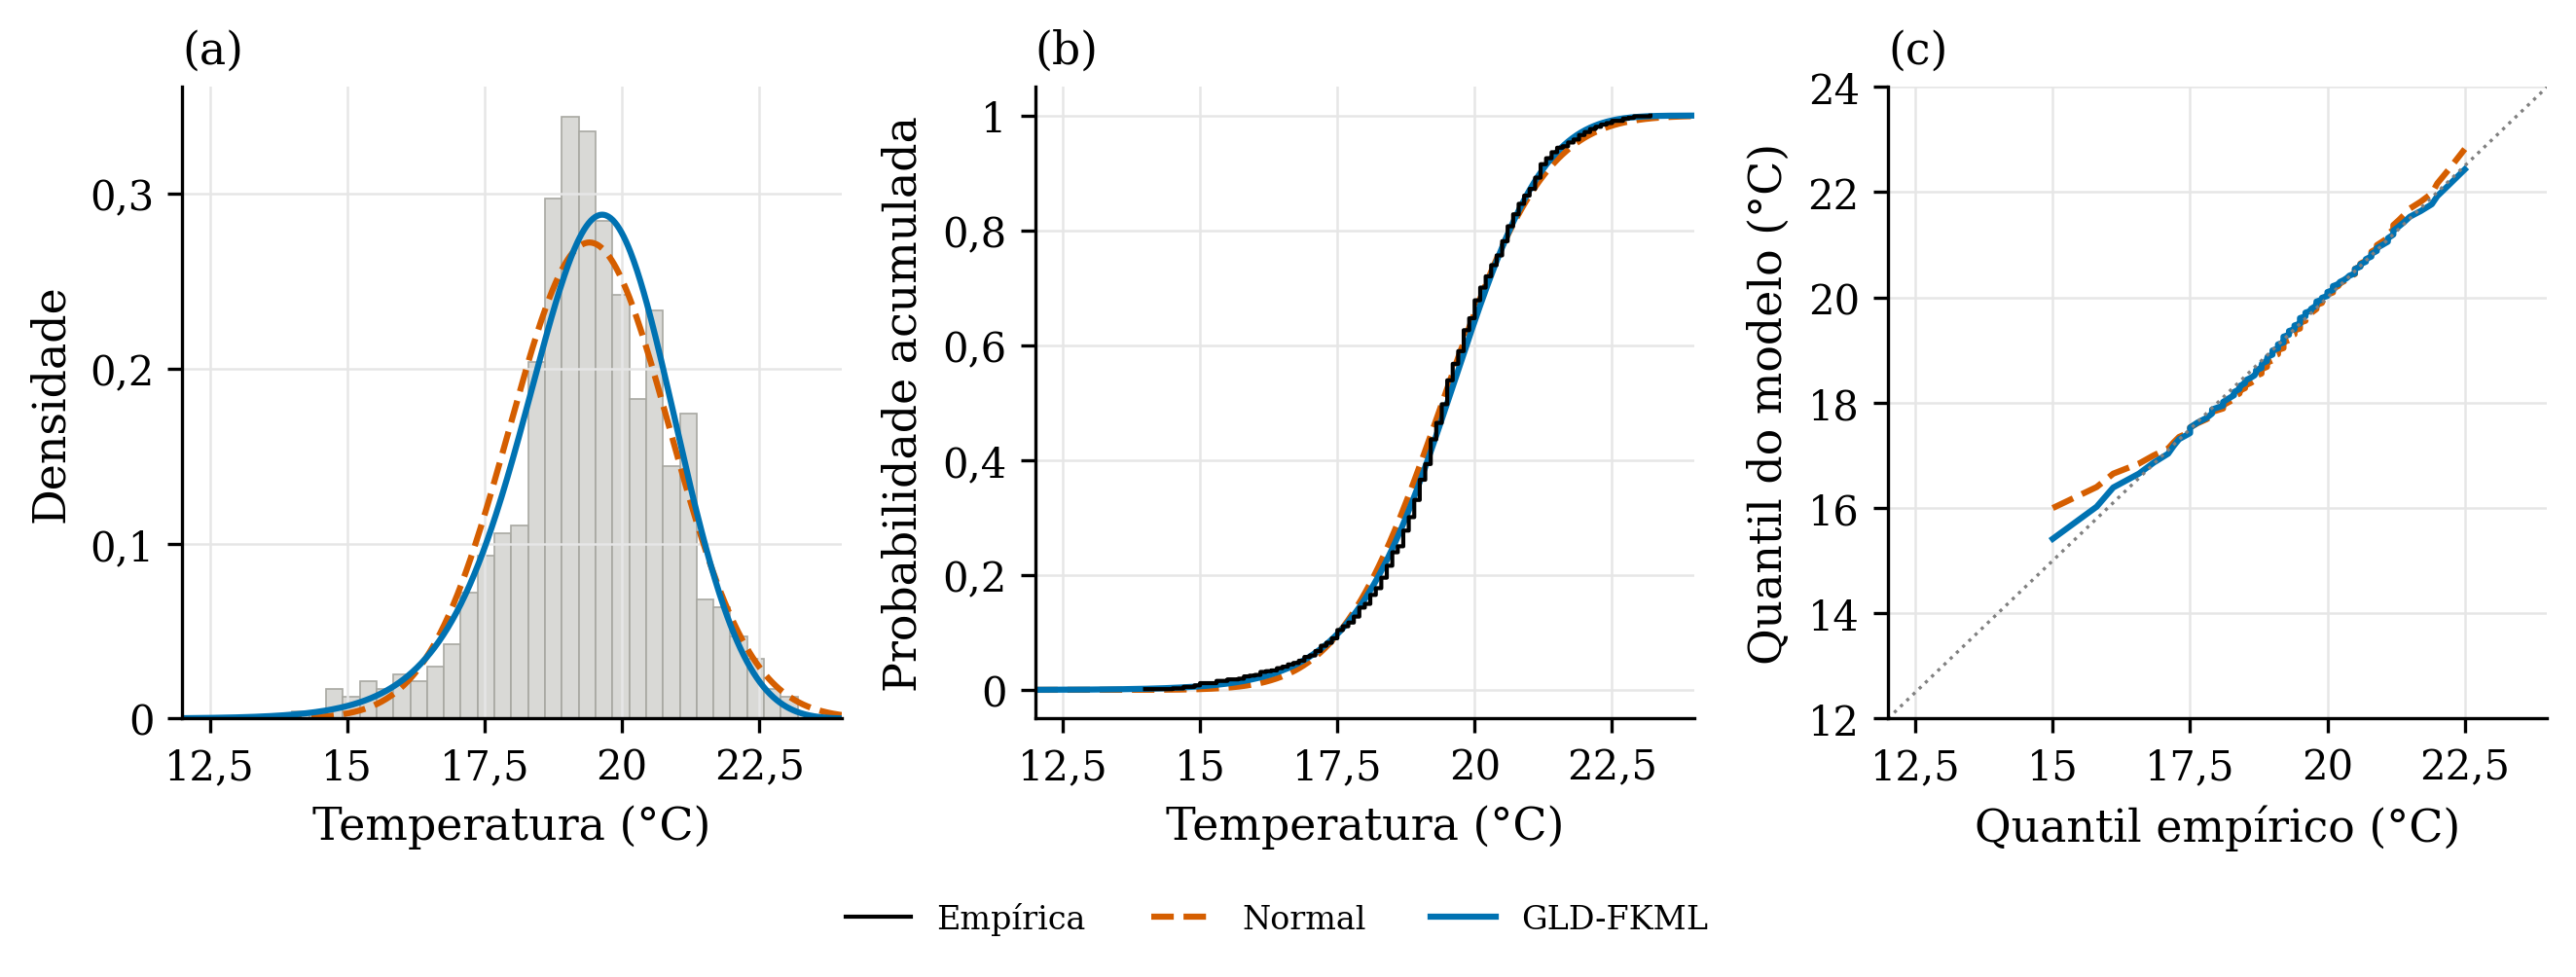
\includegraphics[width=\textwidth]{figura5_temperatura_diagnosticos_pt.png}
\caption{Diagnóstico comparativo das temperaturas de julho, com (a) densidades sobrepostas ao histograma, (b) funções distribuição acumuladas e (c) gráfico quantil-quantil, em que a linha pontilhada indica concordância perfeita.}
\label{fig:diagnosticos_temperatura}
\end{figure}

\subsection{Interpretação didática e física}

A análise dos resultados conduz a uma reflexão conceitual sobre o princípio da parcimônia (navalha de Ockham) no tratamento de dados físicos. A distribuição normal ajustada exibe uma distância de Kolmogorov-Smirnov pequena ($D_n = 0,064$), e os desvios quantílicos situam-se na ordem de décimos de grau Celsius ($+0,16\,^\circ\text{C}$ no quantil de 5\% e $+0,12\,^\circ\text{C}$ no de 95\%).

Para decidir se essas discrepâncias justificam um modelo mais complexo, a escala adequada não é a incerteza do sensor, que afeta cada leitura e pouco altera a forma da distribuição das médias diárias, mas a incerteza amostral dos próprios quantis empíricos. Simulando amostras independentes de $768$ valores a partir da GLD ajustada, o desvio padrão do quantil empírico de $5\%$ é de cerca de $0{,}15\,^\circ\text{C}$, e o do quantil de $95\%$, de cerca de $0{,}09\,^\circ\text{C}$. Temperaturas de dias consecutivos, porém, são fortemente correlacionadas (coeficiente de autocorrelação de $0{,}65$), e julhos de anos diferentes podem ser sistematicamente mais frios ou mais quentes, de modo que a amostra contém menos informação independente do que sugerem os $768$ valores. Reamostrando anos inteiros por \textit{bootstrap}, o que preserva essas duas fontes de dependência, os desvios padrão dos quantis de $5\%$, $50\%$ e $95\%$ passam a $0{,}38$, $0{,}10$ e $0{,}21\,^\circ\text{C}$. As discrepâncias da normal ($+0{,}16$, $-0{,}09$ e $+0{,}12\,^\circ\text{C}$) estão, portanto, dentro da incerteza com que os próprios quantis são conhecidos. Já o valor de $D_n$ da normal, cerca do dobro do valor crítico de $5\%$ do teste de Lilliefors para observações independentes ($0{,}886/\sqrt{n} \approx 0{,}032$)~\cite{lilliefors1967}, sugere uma diferença de forma; mas a dependência entre dias torna esse valor crítico otimista, e o resultado não é conclusivo. Nesses casos, mesmo que a GLD-FKML acomode a assimetria negativa e reduza $D_n$ para $0{,}041$, com desvios quantílicos abaixo de $0{,}06\,^\circ\text{C}$, o acréscimo de dois parâmetros livres exige julgamento crítico, pois, para muitas aplicações térmicas usuais, o modelo normal de dois parâmetros oferece uma descrição simples, robusta e aceitável.

O suporte da GLD ajustada reforça essa leitura. Com $\lambda_3$ e $\lambda_4$ positivos, o modelo é limitado nos dois lados, entre $-33,9\,^\circ\text{C}$ e $24,6\,^\circ\text{C}$. O limite superior é plausível, pouco acima do máximo observado de $23,2\,^\circ\text{C}$; o inferior é fisicamente implausível para Brasília em julho, embora o modelo atribua a essa região uma probabilidade desprezível, porque $\lambda_3$ muito pequeno produz uma cauda esquerda longa e extremamente fina. Os limites do suporte, portanto, são uma consequência matemática dos parâmetros, e não devem ser lidos como limites físicos da grandeza.

Por outro lado, caso o foco resida na estimativa de eventos de frio intenso (cauda esquerda), a assimetria negativa capturada pela GLD ganha relevância. Essa assimetria tem uma origem física identificável: no inverno do Brasil Central, a passagem ocasional de frentes frias e a incursão de massas de ar polar produzem dias isolados bem mais frios que a média, sem um mecanismo equivalente que produza dias anormalmente quentes na mesma proporção. A estatística descreve a cauda; a meteorologia explica por que ela existe. É imperativo frisar aos estudantes que os quantis estimados descrevem a variabilidade das temperaturas médias diárias no histórico observado do mês; não representam intervalos de confiança da média amostral, nem limites do sensor, tampouco uma previsão para um dia específico.

\subsection{Por que não a precipitação?}

A justificativa pedagógica para a escolha da temperatura em detrimento de grandezas como a precipitação evidencia cuidados indispensáveis na modelagem empírica, discutidos a seguir.

\begin{enumerate}
    \item \textbf{Precipitação diária:} na série histórica, de $8.759$ valores válidos, $5.675$ são exatamente iguais a zero (dias sem chuva). Variáveis com massa de probabilidade concentrada na origem não podem ser representadas diretamente por uma única densidade contínua; exigiriam um modelo misto (uma parte para a ocorrência de chuva e uma densidade contínua para os dias chuvosos), introduzindo uma complexidade alheia ao objetivo didático central do artigo.
    \item \textbf{Máximos anuais de chuva e o modelo de Gumbel:} a teoria de valores extremos frequentemente associa máximos em blocos à distribuição de Gumbel. Todavia, uma série de 25 anos fornece no máximo 25 máximas anuais, e ajustar quatro momentos de uma distribuição flexível a uma amostra desse tamanho resulta em estimadores de variância elevada. Além disso, falhas de registro introduzem uma incerteza importante, pois o dia faltante pode ser precisamente o da máxima anual.
\end{enumerate}

Assim, a temperatura média diária no recorte de julho constitui um exemplo didático adequado, com dados contínuos, amostra expressiva ($n = 768$) e simetria aproximada suficiente para contrastar a virtude da simplicidade analítica com o custo da flexibilidade paramétrica.
